\onecolumn
\chapter{Auswertung}
\label{ch:auswertung}

\section*{Fehlerrechnung}
Für die statistische Auswertung von $n$ Messwerten $x_i$ werden folgende Größen definiert \cite{errorSkript25}:
\begin{align}
    \bar{x} &= \frac{1}{n} \sum_{i=1}^{n} x_i \vphantom{\sqrt{\sum_i^n}^2} && \text{\textcolor{gray}{Arithmetisches Mittel}} \label{eq:arithmetisches_mittel} \\
    \sigma^2 &= \frac{1}{n-1} \sum_{i=1}^{n} (x_i - \bar{x})^2 \vphantom{\sqrt{\sum_i^n}^2} && \text{\textcolor{gray}{Variation}} \label{eq:variation} \\
    \sigma &= \sqrt{\frac{1}{n-1} \sum_{i=1}^{n} (x_i - \bar{x})^2} \vphantom{\sqrt{\sum_i^n}^2} && \text{\textcolor{gray}{Standardabweichung}} \label{eq:standardabweichung} \\
    \Delta \bar{x} &= \frac{\sigma}{\sqrt{n}} = \sqrt{\frac{1}{n(n-1)} \sum_{i=1}^n(\bar x - x_i)^2} \vphantom{\sqrt{\sum_i^n}^2} && \text{\textcolor{gray}{Fehler des Mittelwerts}} \label{eq:fehler_mittelwert} \\
    \Delta f &= \sqrt{\left(\frac{\partial f}{\partial x} \Delta x\right)^2 + \left(\frac{\partial f}{\partial y} \Delta y\right)^2} \vphantom{\sqrt{\sum_i^n}^2} && \text{\textcolor{gray}{Gauß’sches Fehlerfortpflanzungsgesetz für $f(x,y)$}} \label{eq:gauss_fehlfortpflanzung} \\
    \Delta f &= \sqrt{(\Delta x)^2 + (\Delta y)^2} \vphantom{\sqrt{\sum_i^n}^2} && \text{\textcolor{gray}{Fehler für $f = x + y$}} \label{eq:fehler_summe} \\
    \Delta f &= |a| \Delta x \vphantom{\sqrt{\sum_i^n}^2} && \text{\textcolor{gray}{Fehler für $f = ax$}} \label{eq:fehler_proportional} \\
    \frac{\Delta f}{|f|} &= \sqrt{\left(\frac{\Delta x}{x}\right)^2 + \left(\frac{\Delta y}{y}\right)^2} \vphantom{\sqrt{\sum_i^n}^2} && \text{\textcolor{gray}{relativer Fehler für $f = xy$ oder $f = x/y$}} \label{eq:relativer_fehler} \\
    \sigma &= \frac{|a_{lit} - a_{gem}|}{\sqrt{\Delta a_{lit}^2 + \Delta a_{gem}^2}} \vphantom{\sqrt{\sum_i^n}^2} && \text{\textcolor{gray}{Berechnung der signifikanten Abweichung}} \label{eq:signifikante_abweichung}
\end{align}

\twocolumn


% /////////////// Aufgabe 1 ///////////////
\section{Aufgabe 1: Qualitative Beobachtung der drei Zylinder}
Die Messung zeigte, dass beim gleichzeitigen Start der drei Rollkörper der Verbundzylinder 
zuerst und der Hohlzylinder zuletzt das Ende der schiefen Ebene erreichte. 
Ursache hierfür ist das unterschiedliche Trägheitsmoment der Körper. 
Da alle nahezu die gleiche Masse besitzen, entscheidet die Massenverteilung über das Trägheitsmoment: 
Beim Hohlzylinder liegt die Masse weiter von der Rotationsachse entfernt, wodurch sein 
Trägheitsmoment gemäß \hyperref[eq:traegheit_hohl]{Gleichung \ref*{eq:traegheit_hohl}} größer ist. 
Beim Verbundzylinder ist die Masse hingegen näher an der Achse konzentriert, was zu einem kleineren Trägheitsmoment als beim Vollzylinder führt 1
(vgl. \hyperref[eq:traegheit_voll]{Gleichung \ref*{eq:traegheit_voll}}).

% /////////////// Aufgabe 2 ///////////////

\section{Aufgabe 2: Bestimmung der Rollbeschleunigung}
Zunächst werden die wichtigen Maße der Ebene vermerkt. Die Zylinder beschleunigen dabei über eine Strecke von $l_{r}' = (87,20 \pm 0,05) \, cm$. Die untere Kante der Abrollhöhe liegt bei $h` = (12,70 \pm 0,05) cm$. Wir müssen jedoch noch die Dicke der Holzplatte und der Metallplatte dazu addieren. Die Werte liegen bei $D_h'= (1,8 \pm 0,05) cm$ für die Holzplatte und $D_m'= (0,2 \pm 0,05) cm$ für die Metallplatte.
Der Fehler der gesamt Starthöhe ist nach \hyperref[eq:gauss_fehlfortpflanzung]{Gauß'scher Fehlerfortpflanzung (\ref*{eq:gauss_fehlfortpflanzung})}
\begin{equation}
    \Delta h_s = 0,09 cm
\end{equation}

Unsere Starthöhe liegt somit bei
\begin{equation}
    h_s = (14,70 \pm 0,09)\, cm.
\end{equation}

Um später Ergebnisse besser überprüfen zu können, haben wir auch noch die Projektion der Lauffläche (die Ankathete) vermessen und kamen dabei auf eine Länge von $l_{an}' = (86,00 \pm 0,05) \, cm$.

Da uns alle drei Kantenlängen bekannt sind, können wir den Winkel $\alpha$ sowohl über den $\sin$ als auch den $\cos$ berechnen. 
\begin{align}
    \alpha_{\sin} &= \frac{h_s}{l_r'} \\
    \alpha_{\cos} &= \frac{l_{an}'}{l_r'}.
\end{align}

Die Ungenauigkeiten der beiden Winkel lassen sich über die \hyperref[eq:gauss_fehlfortpflanzung]{Gauß'sche Fehlerfortpflanzung (\ref*{eq:gauss_fehlfortpflanzung})} bestimmen;
\begin{align}
    \Delta \alpha_{\sin} &= \frac{1}{1+\left(\frac{h_s'}{l_r'}\right)^2} \cdot \sqrt{\left(\frac{\Delta h_s'}{l_r'}\right)^2 + \left(\frac{\Delta l_r' \cdot h_s'}{{l_{r}'}^2}\right)^2} \\
    \notag \\
    \Delta \alpha_{\cos} &= \frac{1}{1+\left(\frac{l_{an}'}{l_r'}\right)^2} \cdot \sqrt{\left(\frac{\Delta l_{an}'}{l_r'}\right)^2 + \left(\frac{\Delta l_r' \cdot l_{an}'}{{l_{r}'}^2}\right)^2}.
    \label{eq:fehler_alpha_cos}
\end{align}

Wir wollen nun beide Winkel berechnen. Wichtig dabei ist, das die \hyperref[eq:fehler_alpha_cos]{Gleichungen} den Fehler in $rad$ angeben, dieser wird noch in $deg$ umgerechnet.
\begin{equation}
    \alpha_{deg} = \frac{\alpha_{rad} \cdot 180^\circ}{\pi}.
\end{equation}

Somit sind unsere zwei Winkel
\begin{equation}
\boxed{
    \alpha_{\sin} = (9,66 \pm 0,06) ^\circ
}
\end{equation}
und
\begin{equation}
\boxed{
    \alpha_{\cos} = (9,5163 \pm 0,0229) ^\circ
    \label{eq:alpha_cos}
}.
\end{equation}

Nun wird überprüft, ob die beiden berechneten Winkel sich gegenseitig >>decken<<, diese also statistisch signifikant. Hierfür wurde die Gleichung zur \hyperref[eq:signifikante_abweichung]{Berechnung der signifikanten Abweichung (\ref*{eq:signifikante_abweichung})} genutzt:
\begin{equation}
    \frac{\left| \alpha_{\sin} - \alpha_{\cos} \right|}{\sqrt{(\Delta \alpha_{\sin})^2 + (\Delta \alpha_{\cos})^2}} = 2,24\sigma. 
\end{equation}

Die Werte sind als eher nicht statistisch signifikant einzustufen. Mehr zur Analyse in der \hyperref[ch:diskussion]{Diskussion}. In folgenden Rechnungen wird der Winkel $\alpha_{\cos}$ verwendet, da dieser die kleinere Ungenauigkeit aufweist. Die \hyperref[fig:maße_re]{Abbildung \ref{fig:maße_re}} zeigt die zur Berechnung benutzen Werte.

Die folgende Rechnung wird sich nun mit der Bestimmung der Beschleunigung befassen. Dazu wird \hyperref[eq:traegheit_voll]{Gleichung \ref*{eq:traegheit_voll}} in die \hyperref[eq:beschleunigung]{Gleichung \ref*{eq:beschleunigung}} eingesetzt. Folglich kommt man zum Ausdruck für den Vollzylinder:
\begin{equation}
    a_{voll} = \frac{2}{3} \cdot g \cdot \sin \alpha.
\end{equation}

Die Ungenauigkeit $\Delta a_{voll}$ wird über die \hyperref[eq:gauss_fehlfortpflanzung]{Gauß'sche Fehlerfortpflanzung (\ref*{eq:gauss_fehlfortpflanzung})} bestimmt:
\begin{equation}
    \Delta a_{voll} = \sqrt{\left(\frac{2}{3} g \cos(\alpha) \cdot \Delta \alpha^2\right)^2 + \left(\frac{2}{3}\sin(\alpha) \cdot \Delta g\right)^2}.
\end{equation}

Für die Erdbeschleunigung nutzen wir den Heidelberger Standardwert von $g_{heidelberg} = (9,80984 \pm 0, 00002) \frac{m}{s^2}$ Die Beschleunigung des Vollzylinders ist somit
\begin{equation}
    \boxed{
        a_{voll,lit} = (1,081 \pm 0,003) \frac{m}{s^2}
    }.
    \label{eq:a_v_l}
\end{equation}

Analog wird auch die Beschleunigung des Hohlzylinders bestimmt. In diesem Fall wird jedoch \hyperref[eq:traegheit_hohl]{Gleichung \ref*{eq:traegheit_hohl}} in die \hyperref[eq:beschleunigung]{Gleichung \ref*{eq:beschleunigung}} eingesetzt. Die Beschleunigung ist somit:
\begin{equation}
    a_{hohl} = \frac{2g \sin \alpha}{3+\left(\frac{r}{R}\right)^2}.
    \label{eq:a_h}
\end{equation}

Die Ungenauigkeit der Hohlzylinderbeschleunigung wird via \hyperref[eq:gauss_fehlfortpflanzung]{Gauß'scher Fehlerfortpflanzung (\ref*{eq:gauss_fehlfortpflanzung})} bestimmt:
\begin{equation}
    \Delta a_{\mathrm{hohl}}
    = \sqrt{
    \left( \frac{a_{\mathrm{hohl}}}{\tan\alpha}\,\Delta\alpha \right)^{2}
    + \left( \frac{a_{\mathrm{hohl}}}{g}\,\Delta g \right)^{2}
    + \left( \frac{2\,a_{\mathrm{hohl}}\,r}{R^{2}\,\bigl(3+(r/R)^{2}\bigr)}\,\Delta r \right)^{2}
    + \left( \frac{2\,a_{\mathrm{hohl}}\,r^{2}}{R^{3}\,\bigl(3+(r/R)^{2}\bigr)}\,\Delta R \right)^{2}
    }.
\end{equation}

\newpage

$a_{hohl}$ wird dabei via \hyperref[eq:a_h]{Gleichung \ref*{eq:a_h}} bestimmt. Der Innendurchmesser des Hohlzylinder ist $r = (4,00 \pm 0,05) cm$ und der Außendurchmesser $r = (5,00 \pm 0,05) cm$. Es wird wieder die Erdbeschleunigung für Heidelberg benutzt. Für Alpha wird wieder $\alpha_{\cos}$ eingesetzt, nach \hyperref[eq:alpha_cos]{Gleichung \ref*{eq:alpha_cos}}. Das Ergebnis ist somit:
\begin{equation}
    \boxed{
        a_{hohl,lit} = (0,92 \pm 0,05) \frac{m}{s^2}
    }.
    \label{eq:a_h_l}
\end{equation}

\begin{figure}[!ht]
    \centering
    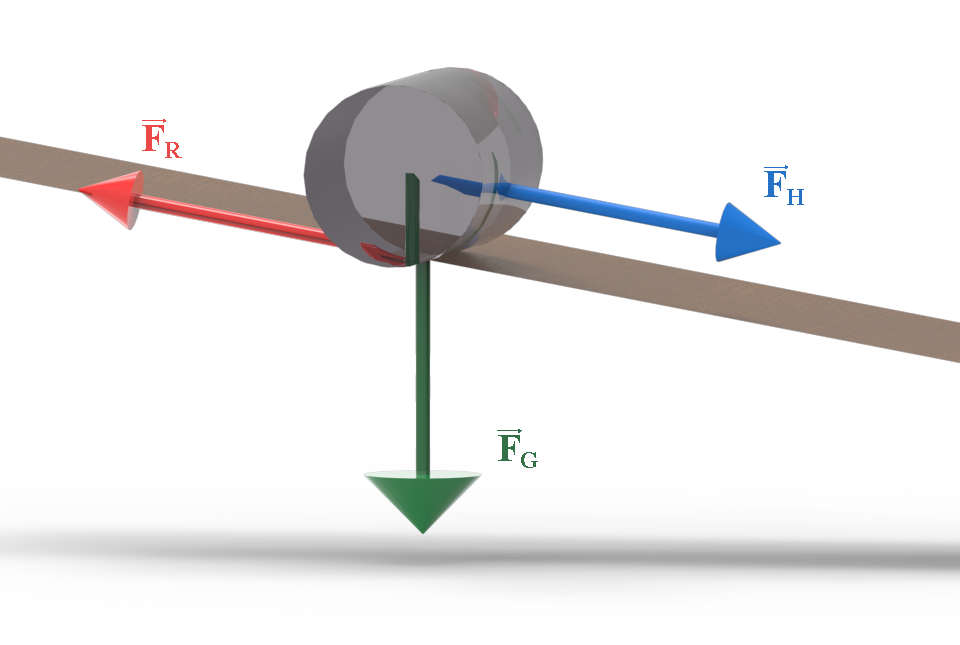
\includegraphics[width=0.45\textwidth]{img/15/Forces.pdf}
    \caption{3D-Rendering der auf einen Zylinder auf einer schrägen Ebene wirkenden Kräfte.}
    \label{fig:zylinder_forces_klein}
\end{figure}

\newpage

% /////////////// Aufgabe 3 ///////////////
\section{Aufgabe 3: Bestimmung der realen Beschleunigung}
Für die folgende Berechnung werden die Daten aus den Tabellen 2 und 3 des \hyperref[Protokoll]{Protokolls} benutzt. Die Lichtschranken (LS) wurden homogen verteilt. Für sowohl den Voll-, als auch den Hohlzylinder wurden je fünf Messungen vorgenommen. Die vier Zeiten der Lichtschranken wurden jeweils notiert. Die Beschleunigung wird dabei grafisch bestimmt. 
Wir wollen aus der Tabelle 3 die Daten der beiden Zylinder betrachten, dafür berechnen wir das \hyperref[eq:arithmetisches_mittel]{Arithmetisches Mittel (\ref*{eq:arithmetisches_mittel})} an jeder Lichtschranken für jeden der Beiden Zylinder. Wir werden die Zeitungenauigkeit über die Standardabweichung $\sigma_i$ für jede der Messungen und betrachten die Ungenauigkeit der Stoppuhr $\Delta t = 0,001s$. Diese Ungenauigkeit ist gerade die Skaleneinheit der Stoppuhr. Die Ungenauigkeit einer Durchschnittlichen Zeit liegt somit bei:
\begin{equation}
    \Delta \overline{t_i} = \sqrt{(\sigma_i)^2 + (\Delta t)^2}.
\end{equation}

Da eine grafische Beschleunigung vorgenommen wird, werden die Mittelwerte quadriert, damit sich eine Gerade zeichnet. Die Ungenauigkeit liegt somit
\begin{equation}
    \Delta ({t_i}^2) = 2 \overline{t_i} \cdot \Delta \overline{t_i}.
\end{equation}

Die Ergebnisse werden \hyperref[tab:mittelwerte]{tabellarisch (\ref*{tab:mittelwerte})} dargestellt.

\begin{table}[!ht]
    \centering
    \hspace*{-2cm}
    \begin{tabular}{c | c | c}
    \toprule
    Messreihe & Vollzylinder & Hohlzylinder \\
    \hline
    $\overline{{t_1}^2}$ [s]& $0,3415 \,\pm\, 0,0024$         & $0,414 \,\pm\, 0,006$ \\
    $\overline{{t_2}^2}$ [s]& $0,650 \,\pm\, 0,005$           & $0,790 \,\pm\, 0,017$ \\
    $\overline{{t_3}^2}$ [s]& $1,027 \,\pm\, 0,008$           & $1,2562 \,\pm\, 0,0215$ \\
    $\overline{{t_4}^2}$ [s]& $1,3689000 \,\pm\, 0,0100220$   & $1,66 \,\pm\, 0,07$ \\
    \bottomrule
    \end{tabular}
    \caption{Messwerte für Vollzylinder (VZ) und Hohlzylinder (HZ) mit Unsicherheiten.}
    \label{tab:mittelwerte}
\end{table}


Die Ungenauigkeit der Strecke liegt bei $\Delta s = 0,05 cm$, was weit unter der Skala des Diagramms liegt (1 Kästchen $\hat = \, 0,4$cm). Dieser Fehler wird daher im folgenden ignoriert.

\begin{figure}[!ht]
    \centering
    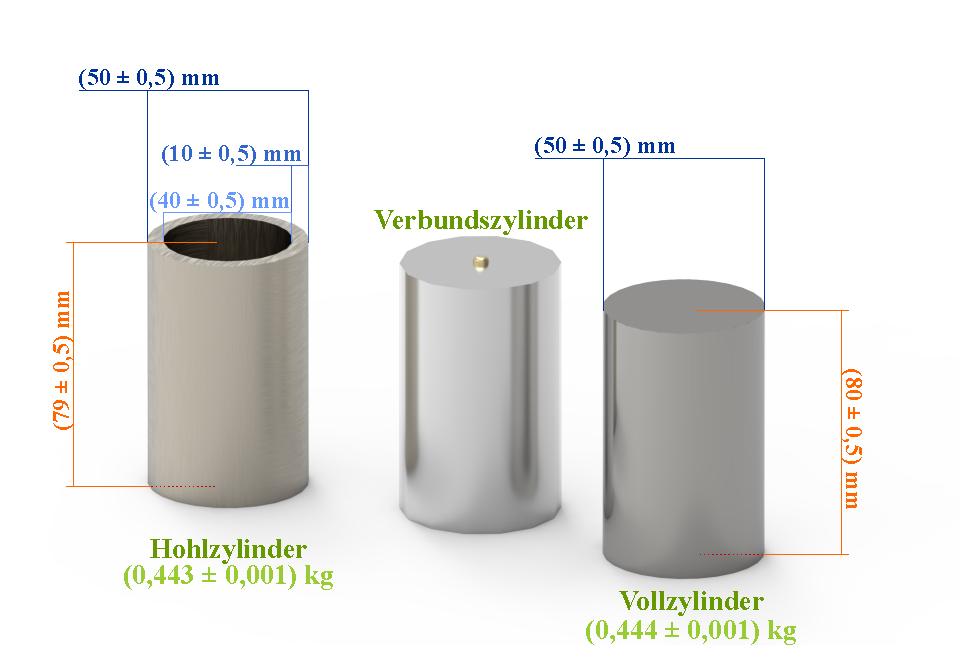
\includegraphics[width=0.45\textwidth]{img/15/Zylindermasse.pdf}
    \caption{3D-Rendering mit den vermessene Größen der Zylinder eingezeichnet (Maßstabsgetreu).}
    \label{fig:zylinder_masse_klein}
\end{figure}


\subsection*{Vollzylinder}
Zunächst wird der Vollzylinder untersucht. Wir wollen seine reale Beschleunigung anhand unserer Messdaten herausfinden. Dazu wird der \hyperref[fig:voll]{Graph \ref*{fig:voll}} betrachtet. Wir werden die Steigungen $\delta s/\delta t^2$ der Ausgleichsgeraden (blau) und der Fehlergeraden (orange) bestimmen. Die Werte sind dem Graphen zu entnehmen. Unsere Steigungen sind somit
\begin{align}
    a_{voll,A} &= 0,4882 \frac{m}{s^2}\\
    a_{voll,F} &= 0,4616 \frac{m}{s^2}.
\end{align}

Die Einheiten wurden angepasst, sodass diese in den typischen SI-Einheiten sind. Die Differenz von $a_{voll,A}$ und $a_{voll,F}$ ist dabei die Ungenauigkeit. Unsere Beschleunigung $a_{voll} = 2 \cdot a_{voll,A}$ für den Vollzylinder liegt daher bei:
\begin{equation}
    \boxed{
        a_{voll} = (0,9764 \pm 0,027) \frac{m}{s^2}
    }.
\end{equation}

Wir wollen dies nun mit dem Wert auf \hyperref[eq:a_v_l]{Gleichung \ref*{eq:a_v_l}} vergleichen. Dazu bestimmen wir die \hyperref[eq:signifikante_abweichung]{signifikante Abweichung (\ref*{eq:signifikante_abweichung})}:
\begin{equation}
    \frac{\left| a_{voll,lit} + a_{voll} \right|}{(\Delta a_{voll,lit})^2 + (\Delta a_{voll})^2} = 3,85\sigma.
\end{equation}

Somit lässt sich dieses Ergebnis als nicht statistisch signifikant einstufen. In der \hyperref[ch:diskussion]{Diskussion} wird darauf genaue eingegangen.

\subsection*{Hohlzylinder}
Die Rechnung läuft analog zur Berechnung des Vollzylinders. Die Steigungen liegen bei:
\begin{align}
    a_{hohl,A} &= 0,3506 \frac{m}{s^2} \\
    a_{hohl,F} &= 0,3631 \frac{m}{s^2}.
\end{align}

Somit ist die Hohlzylinderbeschleunigung
\begin{equation}
\boxed{
    a_{hohl} = (0,7012 \pm 0,0125) \frac{m}{s^2}
}.
\end{equation}

Wir vergleichen mit dem Wert aus \hyperref[eq:a_h_l]{Gleichung \ref*{eq:a_h_l}}:
\begin{equation}
    \frac{\left| a_{hohl,lit} - a_{hohl} \right|}{\sqrt{(\Delta a_{hohl,lit})^2 + (\Delta a_{hohl})^2}} = 4,25\sigma.
\end{equation}

Auch dieser Wert ist nicht statistisch signifikant im Vergleich zu den berechneten Werten aus Aufgabe 2.


\onecolumn
\subsubsection*{Plot der Strecke gegen die Quadratzeit für den Vollzylinder}
\begin{figure}[!ht]
    \centering
    \hspace*{-2.35cm}
    \includegraphics[width=1.3\textwidth, page=3]{Protokolle/15/Chapter/Messprotokoll}
    \caption{Graph für den Vollzylinder. Zurückgelegte Strecke $s$ gegen die Quadratzeit $t^2$. Blau ist die Ausgleichsgerade und orange die Fehlergerade.}
    \label{fig:voll}
\end{figure}

\newpage
\subsubsection*{Plot der Strecke gegen die Quadratzeit für den Hohlzylinder}
\begin{figure}[!ht]
    \centering
    \hspace*{-2.35cm}
    \includegraphics[width=1.3\textwidth, page=4]{Protokolle/15/Chapter/Messprotokoll}
    \caption{Graph für den Hohlzylinder. Zurückgelegte Strecke $s$ gegen die Quadratzeit $t^2$. Blau ist die Ausgleichsgerade und orange die Fehlergerade.}
    \label{fig:hohl}
\end{figure}

\twocolumn

% /////////////// Aufgabe 4 ///////////////
\section{Aufgabe 4: Energien der Zylinder}
Nun wird die Beschleunigung beider Zylinder über den Energieansatz bestimmt. Dazu wird zunächst der Fehler der \hyperref[eq:epot]{Potenziellen Energie (\ref*{eq:epot})} bestimmt:
\begin{equation}
    \Delta E_{pot} = \sqrt{\left(mg \cdot \Delta h \right)^2 + \left(mh \cdot \Delta g \right)^2 + \left(hg \cdot \Delta m \right)^2}
\end{equation}

Die Messwerte, die in dieser Rechnung verwendet werden, sind den Tabellen 1 und 4 des \hyperref[Protokoll]{Protokolls} zu entnehmen. Die Massen unserer Zylinder Schwerpunktgeschwindigkeit
\begin{align}
    m_{voll} &= (444 \pm 1) g \\
    m_{hohl} &= (443 \pm 1) g.
\end{align}



Der Höhennullpunkt ist die Plattenhöhe der Ebene.

Die translatorische Energie eines Körpers berechnet sich über \hyperref[eq:etrans]{Gleichung \ref*{eq:etrans}}. Seine Ungenauigkeit wird über die \hyperref[eq:gauss_fehlfortpflanzung]{Gauß'sche Fehlerfortpflanzung (\ref*{eq:gauss_fehlfortpflanzung})} bestimmt.
\begin{equation}
    \Delta E_{tans} = \sqrt{\left(\frac{v^2}{2} \cdot \Delta m\right)^2 + \left(m\cdot v \cdot \Delta v \right)^2}.
\end{equation}

Es sind wieder fünf Messungen für jeden der Beiden Zylinder gemacht wurden. Wir haben wieder 4 Lichtschranken (LS) aufgestellt, jedoch nur die LS3 und LS4 sind auf der Ebene befestigt wurden. LS1 und LS2 dienen zur Überprüfung der Beschleunigung. Über die gemessenen Zeiten der LS3 und LS4 lässt sich die Endgeschwindigkeit bestimmen. Die Distanz der beiden Lichtschranken lag bei $\delta LS_{Ebene} = 16 cm$. Wir werden die Zylinder wieder nacheinander betrachten.

\subsection*{Vollzylinder}
Die potentielle Energie des Vollzyliders liegt also bei 
\begin{equation}
\boxed{
    E_{pot,voll} = (0,5532 \pm 0,0025)\, J
}.
\end{equation}
Als nächstes wird die Geschwindigkeit des Vollzylinders bestimmt. Dazu werden die Werte aus \hyperref[tab:Vollzylinder_ls]{Tabelle \ref*{tab:Vollzylinder_ls}} genutzt. $\delta\overline{t}$ ist dabei der Mittelwert der Zeitdifferenzen von LS3 und LS4. Die mittlere Geschwindigkeit ist somit
\begin{equation}
    v = \frac{\delta s}{\overline{\delta t}}.
\end{equation}

Über die \hyperref[eq:gauss_fehlfortpflanzung]{Gauß'sche Fehlerfortpflanzung (\ref*{eq:gauss_fehlfortpflanzung})} bestimmen wir die Ungenauigkeit der Geschwindigkeit:
\begin{equation}
    \Delta v =  \sqrt{\left(\frac{\Delta s}{\overline{\delta t}}\right)^2 +\left(\frac{\Delta \overline{\delta t} \cdot s}{\overline{\delta t} ^2}\right)^2}.
\end{equation}

$\Delta \overline{\delta t}$ ist dabei der \hyperref[eq:fehler_mittelwert]{Fehler des Mittelwerts (\ref*{eq:fehler_mittelwert})}. Für unseren Vollzylinder bekommen wir somit eine Endgeschwindigkeit von 
\begin{equation}
    \boxed{
        v_{voll} = (0,65094 \pm 0,00226) \, \frac{m}{s}
    }.
\end{equation}



Somit hat unser Vollzylinder eine Translationsenergie von
\begin{equation}
    \boxed{
        E_{trans,voll} = (0,0941 \pm 0,0007) \, J
    }.
\end{equation}

Zuletzt wollen wir noch die \hyperref[eq:erot]{Rotationsenergie (\ref*{eq:erot})} betrachten. Wir stellen dafür \hyperref[eq:rollbedingung]{Gleichung \ref*{eq:rollbedingung}} nach $\omega$ um:
\begin{equation}
    \omega = \frac{v}{r}.
\end{equation}

Wir setzen zusätzlich $I_{voll}$ nach \hyperref[eq:traegheit_hohl]{Gleichung \ref*{eq:traegheit_hohl}} Damit ist die Rotationsenergie:
\begin{equation}
    E_{rot,voll} = \frac{1}{4} \cdot m \cdot v^2.
\end{equation}

Die Ungenauigkeit beläuft sich auf
\begin{equation}
    \Delta E_{rot,voll} = \sqrt{\left(\frac{v^2}{4} \cdot \Delta m\right)^2 + \left(\frac{v\cdot m}{2} \cdot \Delta v\right)^2}.
\end{equation}

Für unseren Vollzylinder ist die Rotationsenergie somit
\begin{equation}
\boxed{
    E_{rot,voll} = (0,0470 \pm 0,0003) \, J
}
\end{equation}

\begin{table}[!ht]
    \centering
    \begin{tabular}{c | c | c | c}
    \toprule
    Messung & LS3 [s] & LS4 [s] & $\delta$LS [s] \\
    \hline
    1 & 1,392 & 1,637 & 0,245 \\
    2 & 1,383 & 1,630 & 0,247 \\
    3 & 1,384 & 1,630 & 0,246 \\
    4 & 1,395 & 1,641 & 0,246 \\
    5 & 1,392 & 1,637 & 0,245 \\
    \hline
    Durchschnitt &     &     & \textbf{0,2458} \\
    \bottomrule
    \end{tabular}
    \caption{Messwerte für den Vollzylinder mit den Differenzen zwischen LS3 und LS4. $\Delta LS3,LS4 = 0,001s$}
    \label{tab:Vollzylinder_ls}
\end{table}



\subsection*{Hohlzylinder}
Potentielle Energie und translatorische Energie werden analog zum Vollzylinder bestimmt. Somit liegt die potentielle Energie
Die Daten für die Berechnung sind der \hyperref[tab:hohlzylinder_ls]{Tabelle \ref*{tab:hohlzylinder_ls}} zu entnehmen.

\begin{table}[!ht]
    \centering
    \begin{tabular}{c | c | c | c}
    \toprule
    Messung & LS3 [s] & LS4 [s] & $\delta$LS [s] \\
    \hline
    1 & 1,534 & 1,812 & 0,278 \\
    2 & 1,527 & 1,804 & 0,277 \\
    3 & 1,540 & 1,818 & 0,278 \\
    4 & 1,556 & 1,835 & 0,279 \\
    5 & 1,558 & 1,836 & 0,278 \\
    \hline
    Durchschnitt &     &     & \textbf{0,278} \\
    \bottomrule
    \end{tabular}
    \caption{Messwerte für den Hohlzylinder mit den Differenzen zwischen LS3 und LS4. $\Delta LS3,LS4 = 0,001s$}
    \label{tab:hohlzylinder_ls}
\end{table}


Aus diesen berechnet sich die Geschwindigkeit des Hohlzylinders:
\begin{equation}
\boxed{
    v_{hohl} = (0,5755 \pm 0,0019) \, \frac{m}{s}
}
\end{equation}

\begin{equation}
\boxed{
    E_{pot,hohl} = (0,552 \pm 0,004) \, J
},
\end{equation}
und die Translationsenergie
\begin{equation}
\boxed{
    E_{trans,hohl} = (0,0734 \pm 0,0005) \, J
}.
\end{equation}

Zur Bestimmung der Rotationsenergie wird \hyperref[eq:traegheit_hohl]{Gleichung \ref*{eq:traegheit_hohl}} in \hyperref[eq:erot]{Gleichung \ref*{eq:erot}} eingesetzt. Damit kommt man auf
\begin{equation}
    E_{rot,hohl} = \frac{1}{4} m \cdot v^2 \cdot \left(\frac{r^2}{R^2} + 1\right).
\end{equation}

Die Ungenauigkeit nach der \hyperref[eq:gauss_fehlfortpflanzung]{Gauß'schen Fehlerfortpflanzung (\ref*{eq:gauss_fehlfortpflanzung})} liegt bei:

\begin{align}
\Delta E_{\text{rot,hohl}}
= \sqrt{\begin{aligned}
   &\left( \tfrac{1}{4} v^{2}\left(\tfrac{r^{2}}{R^{2}}+1\right)\Delta m \right)^{2} \\
+  &\left( \tfrac{1}{2} m v \left(\tfrac{r^{2}}{R^{2}}+1\right)\Delta v \right)^{2} \\
+  &\left( \tfrac{1}{2} m v^{2} R^{2} r \,\Delta r \right)^{2} \\
+  &\left( \tfrac{1}{2} m v^{2} r^{2} R \,\Delta R \right)^{2}
\end{aligned}}
\end{align}


Die Rotationsenergie des Hohlzylinders wird somit bei 
\begin{equation}
\boxed{
    E_{rot,hohl} = (0,0602 \pm 0,0004) \, J
}.
\end{equation}

Die kinetische Energie circa der potentiellen Energie entsprechen und etwas kleiner sein.
\begin{equation}
    E_{rot} + E_{trans} = E_{pot}.
\end{equation}

Nun wird das Verhältnis der kinetischen und der potentiellen Energie gezogen, dieses sollte im ideal Fall 1 sein (ohne weitere Reibungs- und Wärmeverluste).

Für den Vollzylinder ist diese Abweichung
\begin{equation}
    \frac{E_{rot,voll} + E_{trans,voll} }{E_{pot,voll}} = 25,5\%.
\end{equation}

Das heißt, gerade einmal 25,5\% der potentiellen Energie wurden in kinetische Energie umgesetzt. Dieser Satz ist definitiv weit unter der Erwartung und wird in der \hyperref[ch:diskussion]{Diskussion} besonders diskutiert.

für den Hohlzylinder sind die Ergebnisse ähnlich daneben:
\begin{equation}
    \frac{E_{rot,hohl} + E_{trans,hohl} }{E_{pot,hohl}} = 24,2\%.
\end{equation}
